\chapter{$\theta_{I}$$_{D}$ of ECL}
\label{chap:THID}


A brief explanation of the parameter $\theta_{ID}$ is necessary, since many of the plots presented here use it as an axis, instead of $\theta$. $\theta_{ID}$ is a value assigned to each ring of crystals, starting from 0 for the first ring of crystals in the forward end-cap of the ECL, and ending at 68 for the last ring of crystals in the backward end-cap. A visual explanation of this is shown in Fig~\ref{fig:thetaID}. $\theta_{ID}$ values from 0-12 are in the forward end-cap, 13-58 are in the barrel, and 59-68 are in the backward end-cap. 

\begin{figure}[htb]
	\centerfloat
		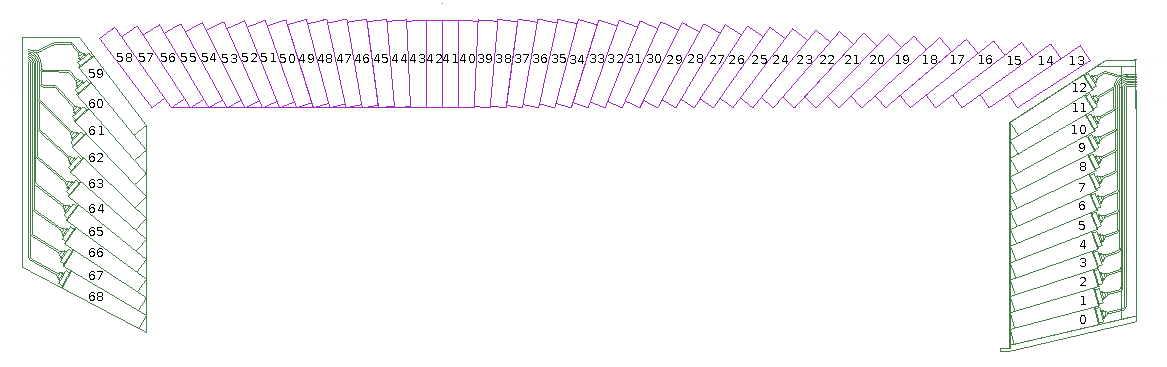
\includegraphics[scale=0.7]{images/ThetaID}
	\caption[$\theta_{ID}$ values for ECL]{$\theta_{ID}$ values for ECL.}	
	\label{fig:thetaID}
\end{figure}

